\documentclass[11pt]{article}
\usepackage[margin=1in]{geometry}
\usepackage[utf8]{inputenc}
\usepackage[T1]{fontenc}
\usepackage{amsmath,amssymb,amsthm}
\usepackage{enumitem}
\usepackage{hyperref}
\usepackage{tikz}
\usetikzlibrary{positioning, arrows.meta}

\newtheorem{definition}{Definition}
\newtheorem{proposition}{Proposition}
\newtheorem{remark}{Remark}

\newcommand{\D}{\mathcal{D}}
\newcommand{\Dm}{\mathcal{D}^{-}}
\newcommand{\Exp}{\mathrm{Exp}}
\newcommand{\Nov}{\mathrm{Nov}}
\newcommand{\Score}{\mathrm{Score}}
\newcommand{\Rob}{\mathrm{Rob}}
\newcommand{\pPartial}{\vdash_{\partial}}
\newcommand{\defto}{\Rightarrow}
\newcommand{\strictto}{\rightarrow}
\newcommand{\defeatto}{\leadsto}
\newcommand{\comp}[1]{\overline{#1}}
\newcommand{\UCB}{\mathrm{UCB1}}

\setlength{\parskip}{6pt}
\setlength{\parindent}{0pt}
\pagestyle{empty}

\begin{document}

\begin{center}
{\Large\bfseries Defeasible Games}\\[4pt]
{\normalsize Patrick Cooper, University of Colorado Boulder}\\[2pt]
\end{center}

\vspace{-4pt}\hrule\vspace{8pt}

\section{Core Idea}

The DeFAb pipeline provides two capabilities that are currently separate: (1)~a preference optimization framework (DPO, RLHF, GRPO) that uses the polynomial-time verifier as a reward signal, and (2)~an adversarial debate framework where MCTS agents compete over derivation trees. The central proposal is to \emph{unify} these: adversarial game outcomes become preference data for DPO, and game dynamics become the environment for RLVR.

The key object is a \emph{defeasible conflict}: a theory $\D$ where two rules produce contradictory conclusions. The game is to resolve the conflict by constructing a defeater.

\subsection*{Philosophical Foundation}

This game formulation operationalizes a specific account of how knowledge advances. Popper~\cite{popper1959logic} argued that scientific theories earn their status by surviving attempts at falsification. In our formalization, defeasible rules are Popperian conjectures: revisable claims that make predictions and expose themselves to refutation. Defeaters are falsifiers: structured counterevidence that overrides specific defaults.

Lakatos~\cite{lakatos1976proofs} refined this picture for mathematics in \emph{Proofs and Refutations}. Mathematical knowledge develops through a dialectical cycle: a conjecture is proposed (the defeasible rule), a counterexample is discovered (the anomaly), and the conjecture is refined by restricting its scope or adding conditions (the conservative defeater). Lakatos identified specific strategies for this refinement: ``monster-barring'' (excluding the counterexample from the conjecture's domain), ``exception-barring'' (adding conditions that rule out the counterexample class), and ``lemma-incorporation'' (absorbing the exception into the theorem's structure). Each of these maps to a distinct type of defeater construction in our framework, and the conservativity requirement ensures that whichever strategy the model adopts, the valid core of the original conjecture is preserved.

The defeasible conflict game makes this dialectic adversarial. Two agents compete to determine which resolution of a conflict is formally superior. This is Lakatos's seminar room, formalized: participants propose competing refinements and the proof (the verifier) adjudicates.

\section{Defeasible Conflict Games}

\begin{definition}[Defeasible Conflict]
A defeasible conflict in theory $\D$ is a pair of defeasible rules $(r_A, r_B)$ such that $\D \pPartial q$ via a chain including $r_A$ and $\D \pPartial \comp{q}$ via a chain including $r_B$, with no existing superiority relation resolving the conflict.
\end{definition}

\begin{definition}[Conflict Resolution Game]
Given a conflict $(r_A, r_B, q)$ over theory $\D$, a two-player game proceeds as follows:
\begin{enumerate}[nosep]
    \item \textbf{Player A} uses MCTS over the derivation space to construct a defeater $d_A$ such that $\D \cup \{d_A\} \pPartial q$ and $\D \cup \{d_A\} \not\pPartial \comp{q}$. That is, $d_A$ resolves the conflict in favor of $r_A$.
    \item \textbf{Player B} does the same for $r_B$: constructs $d_B$ such that $\D \cup \{d_B\} \pPartial \comp{q}$ and $\D \cup \{d_B\} \not\pPartial q$.
    \item Both defeaters are scored by the polynomial-time verifier for:
    \begin{itemize}[nosep]
        \item Resolution: does the defeater actually resolve the conflict?
        \item Conservativity: $|\Exp(\D \cup \{d\}) \setminus \Exp(\D)| + |\Exp(\D) \setminus \Exp(\D \cup \{d\})|$
        \item Novelty: $\Nov(d, \D)$
    \end{itemize}
    \item The \textbf{winner} is the player whose defeater achieves higher composite score: resolution (binary gate) $\times$ conservativity (lower is better) $\times$ novelty bonus.
\end{enumerate}
\end{definition}

\section{DPO via Game Outcomes}

Standard DPO constructs preferences by sampling model responses and scoring them. The game formulation replaces this with structurally grounded preferences:

\begin{definition}[Game-Generated Preference Pair]
Given a conflict $(r_A, r_B, q)$ with game outcome $(d_w, d_l)$ where $d_w$ is the winning defeater and $d_l$ the losing defeater:
\[
    (y_w, y_l) = \bigl(\rho_{\mathrm{enc}}(d_w),\; \rho_{\mathrm{enc}}(d_l)\bigr)
\]
where $\rho_{\mathrm{enc}}$ renders the defeater in the prompt modality. The preference reflects which resolution is formally superior, independent of any model's behavior.
\end{definition}

The margin-weighted DPO loss applies directly, with $\Delta r_{wl}$ now representing the composite score gap between game outcomes rather than sampled response scores.

Three properties distinguish game-generated preferences from sampling-based preferences:

\begin{enumerate}[nosep]
    \item \textbf{Signal source.} Preferences come from the structure of the defeasible theory, not from model errors. The model is trained on what the knowledge base says is correct, not on its own failure modes.
    \item \textbf{Strategic depth.} MCTS explores the space of possible defeaters with principled exploration-exploitation tradeoffs. A single conflict may admit dozens of valid defeaters at varying conservativity levels. MCTS finds the best ones.
    \item \textbf{Scale.} The number of preference pairs scales with the number of conflicts in the knowledge base. UMLS alone provides tens of thousands of structured conflicts.
\end{enumerate}

\section{RLVR via Defeasible Self-Play}

RLVR replaces learned reward models with verifiable rewards. In the defeasible game setting, RLVR takes two forms.

\subsection{GRPO on Game Instances}

The straightforward extension: use GRPO (group relative policy optimization) on game-generated conflict instances. For each conflict, the model generates $G$ candidate defeaters. Each is scored by the verifier. Advantages are normalized within the group:
\[
    \hat{A}_i = \frac{\Score(d_i, \D, q) - \mathrm{mean}(\mathbf{s})}{\mathrm{std}(\mathbf{s})}
\]
where $\mathbf{s}$ is the vector of verifier scores across all $G$ candidates.

GRPO's sparsity property applies: conflicts where all $G$ candidates receive identical scores produce zero gradient. Learning concentrates on the model's decision boundary, where it produces mixed-quality defeaters.

\subsection{Self-Play}

The model plays both sides. For each conflict $(r_A, r_B, q)$:
\begin{enumerate}[nosep]
    \item Generate $G$ candidate defeaters for Rule A: $\{d_A^1, \ldots, d_A^G\}$
    \item Generate $G$ candidate defeaters for Rule B: $\{d_B^1, \ldots, d_B^G\}$
    \item Score all $2G$ candidates with the verifier
    \item The winning side's best defeater is reinforced; the losing side's best is suppressed
\end{enumerate}

As the model improves at one side, the other side must improve to compete. The difficulty of the game tracks the model's capability without manual curriculum scheduling.

\subsection{Process Reward from Derivation Steps}

The defeasible derivation decomposes into independently verifiable steps:
\begin{enumerate}[nosep]
    \item \textbf{Conflict identification}: Did the model correctly identify the conflicting rules? (Checkable: do both rules exist in $\D$ with contradictory heads?)
    \item \textbf{Attack analysis}: Did the model identify which rules attack the target? (Checkable: enumerate attacking rules via the engine.)
    \item \textbf{Defeater construction}: Is the proposed defeater syntactically well-formed and does it target the correct rule? (Checkable: parse and verify the defeater structure.)
    \item \textbf{Resolution verification}: Does the defeater actually resolve the conflict? (Checkable: run the engine on $\D \cup \{d\}$.)
    \item \textbf{Conservativity check}: Are all unrelated expectations preserved? (Checkable: compare $\Exp(\D)$ and $\Exp(\D \cup \{d\})$.)
\end{enumerate}

Each step provides a binary or graded reward signal. GRPO can normalize advantages at the step level rather than the outcome level, producing credit assignment that identifies exactly where the model's reasoning fails.

\subsection{Theory Construction as RL Environment}

The most ambitious formulation. The defeasible theory is the environment. At each step, the model takes an action:
\begin{itemize}[nosep]
    \item Propose a new defeasible rule
    \item Propose a defeater
    \item Assert a superiority relation
\end{itemize}

The verifier provides immediate reward: did this action resolve an anomaly? Did it introduce a new one? Did it preserve conservativity? The episode ends when all anomalies in a target set are resolved or a step budget is exhausted. The model learns to construct coherent defeasible theories, not just answer questions about them.

\section{Unified Training Pipeline}

\begin{center}
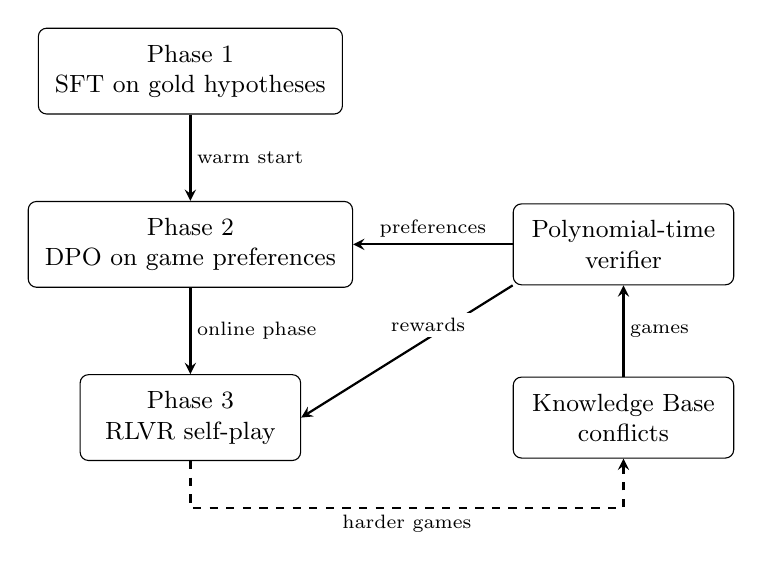
\begin{tikzpicture}[
    >=stealth,
    box/.style={
        draw, rounded corners=3pt,
        minimum height=1cm, minimum width=2.8cm,
        font=\small, inner sep=6pt,
        text centered, align=center
    },
    arr/.style={->, thick},
    lbl/.style={font=\scriptsize, fill=white, inner sep=2pt},
]

% Layout: two columns, left = pipeline (vertical), right = infrastructure (vertical)
% Left column: three training phases stacked vertically
\node[box] (sft) at (0, 0) {Phase 1\\SFT on gold hypotheses};
\node[box] (dpo) at (0, -2.2) {Phase 2\\DPO on game preferences};
\node[box] (rlvr) at (0, -4.4) {Phase 3\\RLVR self-play};

% Right column: verifier and KB
\node[box] (verifier) at (5.5, -2.2) {Polynomial-time\\verifier};
\node[box] (kb) at (5.5, -4.4) {Knowledge Base\\conflicts};

% Pipeline flow (left column, downward)
\draw[arr] (sft) -- node[lbl, right] {warm start} (dpo);
\draw[arr] (dpo) -- node[lbl, right] {online phase} (rlvr);

% Verifier provides preferences to DPO (horizontal)
\draw[arr] (verifier.west) -- node[lbl, above] {preferences} (dpo.east);

% Verifier provides rewards to RLVR (horizontal)
\draw[arr] (verifier.south west) -- node[lbl, above, pos=0.4] {rewards} (rlvr.east);

% KB feeds games into verifier (vertical)
\draw[arr] (kb) -- node[lbl, right] {games} (verifier);

% Feedback loop: RLVR generates harder games back to KB
\draw[arr, dashed] (rlvr.south) -- ++(0, -0.6) -|
    node[lbl, below, pos=0.25] {harder games} (kb.south);

\end{tikzpicture}
\end{center}

Phase 1 (SFT): train on gold hypotheses from existing DeFAb instances. Establishes baseline format compliance and grounding capability.

Phase 2 (DPO): train on game-generated preferences. MCTS pre-computes conflict resolutions offline. The margin-weighted loss internalizes the ordinal structure of conflict resolution quality.

Phase 3 (RLVR): online self-play with GRPO. The model generates defeaters in real time. The verifier provides exact rewards. The feedback loop between model improvement and game difficulty creates an automatic curriculum.

The verifier is the fixed point. It never degrades, never approximates, never drifts. Every training signal, whether preference or reward, is mathematically verified.

\section{Extension to Formalized Mathematics}

The Lakatosian foundation makes the extension to formalized mathematics natural. The isomorphism between DeFAb theories and mathematical proof libraries is precise:

\begin{itemize}[nosep]
    \item \textbf{Strict rules} from proven theorems. \texttt{theorem foo (h1: C1) (h2: C2) : P} becomes $r_s\colon C_1, C_2 \strictto P$, validated by Lean's kernel.
    \item \textbf{Defeasible rules} from weakened theorems. Dropping condition $C_2$ yields $r_d\colon C_1 \defto P$, a conjecture that is usually true but admits exceptions when $C_1 \wedge \neg C_2$ holds.
    \item \textbf{Defeaters} from counterexamples. An instance $a$ with $C_1(a) \wedge \neg C_2(a) \wedge \neg P(a)$ is a falsifier that defeats $r_d$.
    \item \textbf{Conservativity} from the full theorem. The defeater must block $P$ only in the exception region $(\neg C_2)$, preserving every instance where all original conditions hold.
\end{itemize}

The defeasible conflict game applies directly. Two conflicting conjectures (weakened theorems with overlapping but incompatible domains) are resolved by constructing counterexamples that determine which conjecture should yield. Lean serves as the verifier: exact, sound, complete, and requiring no approximation.

\textit{Example.} Euler's formula $V - E + F = 2$. The defeasible rule: this holds for all polyhedra. The defeater: polyhedra with genus $> 0$ (a torus has $V - E + F = 0$). At Level~3, the model must construct the genus-based exception without breaking the formula for convex polyhedra. Lakatos devoted an entire book to the dialectical history of exactly this conjecture.

\textit{Example.} ``Convergent sequences of continuous functions have continuous limits.'' The defeater: pointwise (not uniform) convergence may yield discontinuous limits. The refined conjecture is a strict rule in Mathlib (\texttt{TendstoUniformly.continuous}). The game: Player~A argues for the pointwise convergence conjecture; Player~B constructs the counterexample. The verifier (Lean) confirms the counterexample and checks that the refinement to uniform convergence preserves all valid instances.

\section{Open Questions}

\begin{enumerate}
    \item \textbf{Is RLVF Necessary} Learned preferences via the defeasible games may be adequate and RLVF may not provide tangible benefit. This must be experimentally verified via ablation.
    \item \textbf{How is novelty computed?} We indicate earlier that novelty can be computed, but provide no explicit formulation. There are several clear possibilities which can be tried (Information-theoretic surprisal, topological novelty on the dependency graph), and we must verify a novelty modifier is even required at all. Parsimony or conservativity alone may be sufficient for exploring the decision space.
    \item \textbf{Conflict enumeration at scale.} How many distinct conflicts exist in UMLS, SNOMED, GO? Is the number tractable for exhaustive game generation, or do we need sampling strategies?
    \item \textbf{Game balance.} Are most conflicts ``one-sided'' (one resolution is clearly superior)? If so, the preference signal may be redundant. How many conflicts admit competitive resolutions where MCTS search depth matters?
    \item \textbf{Self-play stability.} Does the self-play dynamic converge, or does it oscillate? The verifier prevents reward hacking, but the model could cycle between favoring Rule A and Rule B without settling.
    \item \textbf{Process vs.\ outcome reward.} Does step-level reward from derivation decomposition actually improve credit assignment, or does the additional complexity of step scoring introduce noise?
    \item \textbf{Transfer to open-ended reasoning.} Models trained on KB-derived conflicts learn to resolve structured disagreements. Does this transfer to open-ended clinical reasoning where the theory is implicit rather than explicit?
    \item \textbf{Connection to drug discovery.} In the biomedical setting, a conflict between ``Drug X treats Condition Y'' and ``Drug X is contraindicated for Comorbidity Z'' is a clinical decision. Can defeasible self-play produce models that reason about pharmacogenomic exceptions without explicit pharmacogenomic training data?
    \item \textbf{Lakatos strategies as reward shaping.} Can the three Lakatosian refinement strategies (monster-barring, exception-barring, lemma-incorporation) be formalized as distinct reward components? If so, the training signal could distinguish \emph{how} the model refines a conjecture, not just whether the refinement is conservative.
    \item \textbf{Mathematics as the cleanest testbed.} Lean provides an exact verifier with no approximation. If the game-based fine-tuning framework works on DeFAb-Math (where verification is perfect), does the approach transfer to biomedical domains (where verification is polynomial-time but operates over noisier knowledge bases)?
    \item \textbf{Popper's asymmetry.} Popper observed that falsification is logically stronger than confirmation: a single counterexample refutes a universal claim, but no number of confirmations can prove one. Does this asymmetry manifest in the game dynamics? Is the opponent (falsifier) systematically advantaged over the proponent (conjecture defender)?
\end{enumerate}

\section{Formal Justification (WIP)}
 
The two-player structure of the conflict resolution game is not a modeling choice. It is forced by the proof theory of defeasible logic. This section makes the argument precise and establishes the formal properties that the training pipeline depends on: binarity, zero-sumness, finiteness, and determinacy.
 
\subsection{From Derivation Conditions to Games}
 
We begin with the standard derivation condition for defeasible provability. In the formulation of Antoniou, Billington, and Governatori~\cite{antoniou2001representation}, the condition $+\partial q$ holds in theory $\D$ if and only if:
 
\begin{enumerate}[nosep]
    \item There exists a rule $r \in R[q]$ such that every antecedent of $r$ is provable, and
    \item For every rule $s \in R[\comp{q}]$ whose antecedents are all provable, there exists a rule $t \in R[q]$ whose antecedents are all provable and $t > s$.
\end{enumerate}
 
The quantifier structure is $\exists \forall \exists$. This alternation defines a two-player evaluation game in the standard sense of logic and model theory. Let the \emph{proponent} control the existential quantifiers and the \emph{opponent} control the universal quantifier. The proponent selects a supporting rule $r$, the opponent selects an attacking rule $s$, and the proponent must counter with a superior rule $t$. A derivation succeeds if and only if the proponent has a winning strategy in this game. This connection between alternating quantifiers and two-player games is not metaphorical; it is the content of the game-theoretic semantics of Hintikka~\cite{hintikka1996principles} applied to the metalanguage of the derivation conditions.
 
\begin{proposition}[Binarity of Defeasible Conflict]\label{prop:binarity}
Let $\D$ be a defeasible theory and let $q$ be a literal. Under classical complementation, every conflict over $q$ in $\D$ partitions the relevant rules into exactly two sets: $R[q]$ and $R[\comp{q}]$. No rule bears on both sides, and no third position exists.
\end{proposition}
 
\begin{proof}
By the definition of a defeasible theory, every rule $r$ has a unique consequent $c(r)$. For a conflict over literal $q$, a rule is relevant if and only if $c(r) = q$ or $c(r) = \comp{q}$. Classical complementation is an involution ($\comp{\comp{q}} = q$), so $c(r) \in \{q, \comp{q}\}$ is an exhaustive and mutually exclusive partition of the relevant rules.
\end{proof}
 
\begin{remark}
Binarity is a consequence of classical negation, not of any domain assumption. A logic with three-valued complementation (e.g., where $q$, $\comp{q}$, and $\bot$ are distinct) could induce three-player conflicts. The restriction to two players is precisely the restriction to classical defeasible logic.
\end{remark}
 
\subsection{From Proof Games to Theory Construction Games}
 
The standard dialogical game operates over a fixed theory: given $\D$, does $+\partial q$ hold? Both the proponent and the opponent select from rules already present in $\D$. Our conflict resolution game (Definition~2) differs in a precise way: the theory is not fixed, and the players construct extensions to it.
 
\begin{definition}[Theory Construction Game]
Let $(r_A, r_B, q)$ be a defeasible conflict in $\D$. The theory construction game $\Gamma(\D, r_A, r_B, q)$ is a simultaneous-move game defined by:
\begin{enumerate}[nosep]
    \item \textbf{Strategy sets.} Player~A's strategy set is $S_A = \{d \in \mathcal{L}_\D \mid \D \cup \{d\} \vdash_\partial q \text{ and } \D \cup \{d\} \not\vdash_\partial \comp{q}\}$. Player~B's strategy set $S_B$ is defined symmetrically. Here $\mathcal{L}_\D$ is the defeater language over $\D$ (defined below).
    \item \textbf{Payoff.} The payoff to Player~A is $u_A(d_A, d_B) = \Score(d_A, \D, q) - \Score(d_B, \D, \comp{q})$, with $u_B = -u_A$.
\end{enumerate}
\end{definition}
 
Two properties of this game require proof: that it is zero-sum, and that it is finite (and therefore determined).
 
\begin{proposition}[Zero-Sum Structure]\label{prop:zerosum}
The theory construction game $\Gamma(\D, r_A, r_B, q)$ is zero-sum.
\end{proposition}
 
\begin{proof}
By construction, $u_B = -u_A$. It remains to show this is not merely a convention but reflects a logical constraint: no theory extension can simultaneously resolve the conflict in favor of both $q$ and $\comp{q}$.
 
Suppose for contradiction that there exists an extension $\D' \supseteq \D$ such that $\D' \vdash_\partial q$ and $\D' \vdash_\partial \comp{q}$ and the conflict $(r_A, r_B)$ is resolved. By the resolution condition (Definition~2), resolution in favor of $q$ requires $\D' \not\vdash_\partial \comp{q}$, and resolution in favor of $\comp{q}$ requires $\D' \not\vdash_\partial q$. Both conditions cannot hold simultaneously. Hence any resolution must favor exactly one side, and the gain of one player is the loss of the other.
\end{proof}
 
\subsection{Finiteness and Determinacy}
 
The standard dialogical game over a fixed theory is finite because defeasible proof trees are well-founded: they bottom out at facts and strict rules. The theory construction game introduces a new concern, since the players are not selecting from a fixed rule set but constructing new rules. The strategy space could in principle be infinite. The following definition and proposition establish that it is not.
 
\begin{definition}[Defeater Language]\label{def:defeater_lang}
Given a defeasible theory $\D$ with predicate signature $\Sigma$ and constant domain $C$, the defeater language $\mathcal{L}_\D$ is the set of all syntactically well-formed defeaters whose predicates are drawn from $\Sigma$, whose constants are drawn from $C$, and whose rule length (number of antecedents) is bounded by $k = \max_{r \in \D} |A(r)|$, the maximum antecedent length of any rule in $\D$.
\end{definition}
 
\begin{proposition}[Finiteness of Strategy Sets]\label{prop:finiteness}
If $\Sigma$ and $C$ are finite, then $\mathcal{L}_\D$ is finite, and therefore $S_A$ and $S_B$ are finite.
\end{proposition}
 
\begin{proof}
A defeater $d$ is specified by: a set of antecedents (a subset of the Herbrand base $\mathrm{HB}(\Sigma, C)$, bounded in size by $k$), a consequent (an element of $\mathrm{HB}(\Sigma, C)$ or its complement), and a target rule in $\D$. Since $\mathrm{HB}(\Sigma, C)$ is finite when $\Sigma$ and $C$ are finite, the number of possible antecedent sets of size at most $k$ is $\sum_{i=0}^{k} \binom{|\mathrm{HB}(\Sigma, C)|}{i}$, which is finite. The number of consequents is $2|\mathrm{HB}(\Sigma, C)|$, and the number of target rules is $|\D|$. The product is finite.
\end{proof}
 
\begin{remark}
The bound $k$ is a modeling choice, not a logical necessity. Without it, the strategy space remains finite (since $\Sigma$ and $C$ are finite, the Herbrand base is finite, and the powerset of a finite set is finite), but the bound ensures the strategy space is computationally manageable. In practice, defeaters in biomedical and mathematical theories rarely exceed the antecedent complexity of the rules they target, so the bound is not restrictive.
\end{remark}
 
\begin{proposition}[Determinacy]\label{prop:determinacy}
The theory construction game $\Gamma(\D, r_A, r_B, q)$ is determined: it has a value $v^*$ such that
\[
    v^* = \max_{d_A \in S_A} \min_{d_B \in S_B} u_A(d_A, d_B) = \min_{d_B \in S_B} \max_{d_A \in S_A} u_A(d_A, d_B).
\]
\end{proposition}
 
\begin{proof}
The game is finite (Proposition~\ref{prop:finiteness}) and zero-sum (Proposition~\ref{prop:zerosum}). By von Neumann's minimax theorem for finite zero-sum games, the game has a value and both players have optimal (possibly mixed) strategies.
\end{proof}
 
\begin{remark}
The simultaneous-move formulation is appropriate because neither player's defeater depends on the other's choice within a single game instance. In the self-play setting (Section~5.2), the same model generates defeaters for both sides independently. The sequential structure arises across training iterations, not within a single game.
\end{remark}
 
\subsection{The Verifier as Fixed Point}
 
The scoring function $\Score(d, \D, q)$ is computed by the polynomial-time verifier. The following property is essential for the training pipeline and distinguishes the defeasible game from settings where reward is learned or approximated.
 
\begin{proposition}[Verifier Invariance]\label{prop:verifier}
The scoring function $\Score$ is:
\begin{enumerate}[nosep]
    \item \textbf{Deterministic:} the same defeater receives the same score on every evaluation.
    \item \textbf{Model-independent:} the score depends only on $d$, $\D$, and $q$, not on the model that generated $d$.
    \item \textbf{Polynomial-time:} for a theory with $n$ rules, scoring requires $O(n^2)$ time via the standard defeasible logic engine.
\end{enumerate}
\end{proposition}
 
These properties jointly guarantee that the game value $v^*$ is stable across training. The minimax strategies may change as the model improves (it may discover new defeaters in $S_A$ or $S_B$ that it previously failed to generate), but the payoff function itself does not drift. This is the precise sense in which the verifier is a fixed point: it defines a stationary game that the model learns to play, rather than a co-evolving objective that the model learns to exploit.
 
\subsection{Lakatos as Extensive Form}
 
The connection to Lakatos~\cite{lakatos1976proofs} can now be stated as a formal claim rather than an analogy.
 
\begin{proposition}[Lakatos Correspondence]\label{prop:lakatos}
Let $\D_{\mathrm{math}}$ be a defeasible theory constructed from a formalized mathematical library (Section~7) where strict rules correspond to proven theorems and defeasible rules correspond to weakened conjectures. Then the Lakatosian dialectical cycle
\[
    \text{conjecture} \longrightarrow \text{counterexample} \longrightarrow \text{refinement}
\]
is the move sequence of a conflict resolution game $\Gamma(\D_{\mathrm{math}}, r_A, r_B, q)$ in which:
\begin{enumerate}[nosep]
    \item The conjecture is the defeasible rule $r_A$ (or $r_B$).
    \item The counterexample is the defeater $d$ constructed by the opposing player.
    \item The refinement is the updated theory $\D_{\mathrm{math}} \cup \{d\}$, which preserves all instances where the original theorem's full conditions hold (conservativity) while blocking the conjecture in the exception region.
\end{enumerate}
When the formalized library is in Lean~4, the verifier is Lean's kernel, which is exact and sound by construction.
\end{proposition}
 
\begin{proof}[Proof sketch]
The correspondence is verified by checking that each component of the Lakatosian cycle satisfies the formal definitions. A weakened theorem (conjecture) is a defeasible rule by Definition~\ref{def:defeater_lang}'s construction in Section~7: dropping a hypothesis $C_2$ from a strict rule $C_1, C_2 \strictto P$ yields the defeasible rule $C_1 \defto P$. A counterexample is an instance $a$ with $C_1(a) \wedge \neg C_2(a) \wedge \neg P(a)$, which constitutes a defeater because it provides evidence for $\comp{P}$ in the scope of $r$'s antecedent. The conservativity condition (Definition~2, item~3) requires that the defeater does not block $P$ in the region where all original hypotheses hold, which is exactly the requirement that the refinement preserve the valid core of the original theorem. The three Lakatosian strategies (monster-barring, exception-barring, lemma-incorporation) correspond to three syntactically distinct classes of defeaters: those that restrict the domain of the defeasible rule, those that add conditions to the antecedent, and those that restructure the rule's dependency chain, respectively.
\end{proof}


\begin{thebibliography}{9}

\bibitem{popper1959logic}
K.~R. Popper.
\newblock \emph{The Logic of Scientific Discovery}.
\newblock Hutchinson, London, 1959.
\newblock Originally published as \emph{Logik der Forschung}, 1934.

\bibitem{antoniou2001representation}
G.~Antoniou, D.~Billington, and G.~Governatori.
\newblock Representation results for defeasible logic.
\newblock \emph{ACM Transactions on Computational Logic}, 2(2):255--287, 2001.
 
\bibitem{hintikka1996principles}
J.~Hintikka.
\newblock \emph{The Principles of Mathematics Revisited}.
\newblock Cambridge University Press, 1996.
 
\bibitem{lakatos1976proofs}
I.~Lakatos.
\newblock \emph{Proofs and Refutations: The Logic of Mathematical Discovery}.
\newblock Cambridge University Press, 1976.

\end{thebibliography}

\end{document}
